\section{Resultados y Mejoras}

Esta sección sintetiza los resultados obtenidos a lo largo del proceso de Diseño Centrado en el Usuario y las mejoras derivadas de la evaluación del prototipo. Los resultados se presentan en tres niveles: los hallazgos de la investigación de usuarios, la respuesta del rediseño a los problemas detectados y las mejoras identificadas tras evaluar el prototipo funcional.

\vspace{0.5cm}
\begin{figure}[H]
\centering
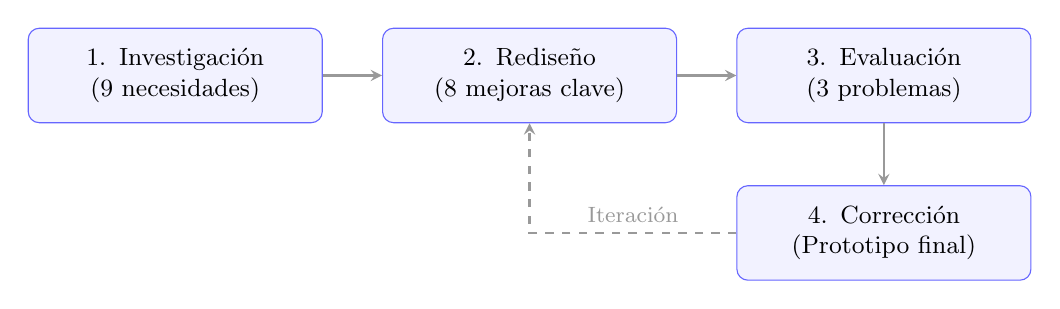
\begin{tikzpicture}[
    box/.style={draw=blue!60, rectangle, rounded corners, minimum width=3.5cm, minimum height=1.2cm, align=center, fill=blue!5, text width=3.5cm, font=\small},
    arrow/.style={->, thick, >=stealth, draw=gray!80}
]
\node[box] (inv) at (0,0) {1. Investigación\\(9 necesidades)};
\node[box] (red) at (4.5,0) {2. Rediseño\\(8 mejoras clave)};
\node[box] (eval) at (9,0) {3. Evaluación\\(3 problemas)};
\node[box] (corr) at (9,-2) {4. Corrección\\(Prototipo final)};

\draw[arrow] (inv) -- (red);
\draw[arrow] (red) -- (eval);
\draw[arrow] (eval) -- (corr);
\draw[arrow, dashed] (corr) -| node[above, near start, font=\footnotesize, text=gray!80] {Iteración} (red);
\end{tikzpicture}
\caption{Ciclo de iteración aplicado en la resolución de problemas de usabilidad.}
\label{fig:ciclo-iteracion}
\end{figure}

\subsection{Resultados de la investigación de usuarios}

La triangulación de encuesta, entrevistas y observación directa permitió caracterizar la experiencia de uso de WebSIS y confirmar que el problema trasciende lo técnico. Entre los hallazgos más relevantes destacan la concentración del uso en periodos críticos, la dificultad percibida en la tarea de inscripción, la alta dependencia de ayuda externa y un impacto emocional sistémico marcado por la ansiedad anticipatoria y la ausencia de confianza en el sistema. Estos hallazgos se tradujeron en nueve necesidades detectadas (N1--N9) y en dos perfiles de usuario claramente diferenciados: el estudiante ingresante y el estudiante regular.

\subsection{Mejoras del rediseño frente a los problemas detectados}

El rediseño propuesto atiende directamente los problemas prioritarios identificados en la evaluación heurística del sistema actual. La siguiente tabla resume cómo cada problema crítico se traduce en una mejora concreta de la interfaz.

{\small
\setlength{\tabcolsep}{4pt}
\renewcommand{\arraystretch}{1.2}
\begin{longtable}{|p{0.9cm}|p{5.5cm}|p{6.5cm}|}
\hline
\textbf{ID} & \textbf{Problema en WebSIS actual} & \textbf{Mejora aplicada en el rediseño} \\
\hline
\endfirsthead

\hline
\textbf{ID} & \textbf{Problema en WebSIS actual} & \textbf{Mejora aplicada en el rediseño} \\
\hline
\endhead

P1 & Ausencia de guía e indicadores de estado en la inscripción. & Flujo de inscripción con estados explícitos (cuenta habilitada, n/máx materias, resumen y estado final). \\
\hline
P2 & Mensajes de error incomprensibles. & Estados y confirmaciones con lenguaje cercano al estudiante e información sobre el siguiente paso. \\
\hline
P3 & Interfaz no responsive, inutilizable en móvil. & Separación por pantallas, accesos compactos y resumen progresivo adaptados a móvil. \\
\hline
P4 & Arquitectura basada en lógica técnica interna. & Estructura reorganizada según las tareas del estudiante, validada con card sorting. \\
\hline
P5 & Falta de confirmación del resultado de las acciones. & Pantalla de estado de inscripción y comprobantes visibles que confirman cada acción. \\
\hline
P6 & Sin acceso directo a tareas frecuentes. & Panel del estudiante con accesos directos a las tareas de mayor uso. \\
\hline
P9 & Etiquetas e íconos ambiguos. & Rotulado alineado al vocabulario del estudiante (pagar matrícula, validar códigos, horario, Kardex). \\
\hline
P10 & Situación académica e información de créditos poco clara. & Kardex con indicadores resumidos y diferenciación entre materias cerradas y en curso. \\
\hline

\caption{Correspondencia entre los problemas detectados y las mejoras del rediseño.}\label{tab:resultados-mejoras}
\end{longtable}
}

La validación de la propuesta con usuarios (card sorting y pruebas sobre wireframes) confirmó que la estructura coincide en gran medida con el modelo mental del estudiante y que los flujos principales pueden completarse sin asistencia. Los puntos de fricción detectados en esa etapa —principalmente la ubicación de la validación de códigos y el cambio de contraseña— permitieron ajustar la visibilidad y el etiquetado de esos accesos antes de avanzar al prototipo.

\subsection{Mejoras aplicadas tras la evaluación del prototipo}

La evaluación del prototipo funcional, mediante pruebas de usabilidad y evaluación heurística, identificó tres problemas que fueron corregidos sobre el propio prototipo, completando un ciclo de iteración. El detalle y las evidencias se encuentran en el Informe de Evaluación; en síntesis:

\vspace{0.5cm}
\begin{figure}[H]
\centering
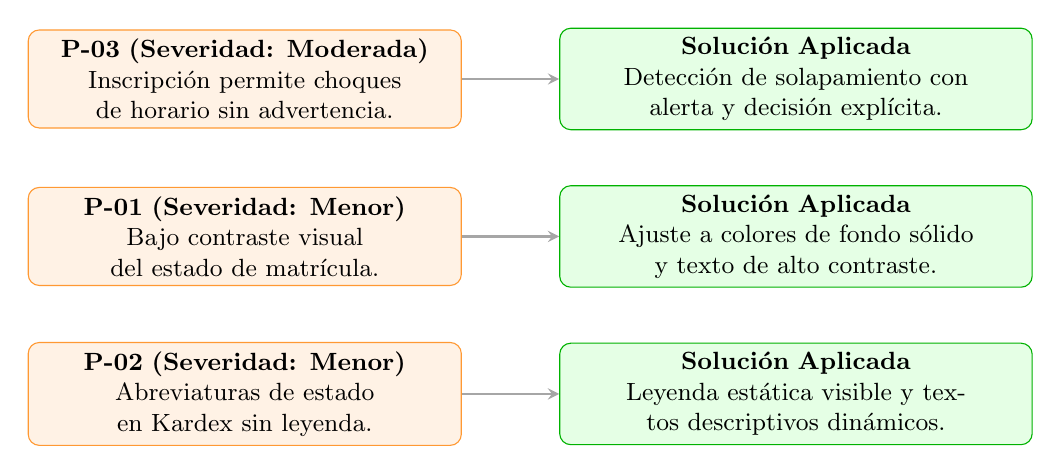
\begin{tikzpicture}[
    prob/.style={draw=orange!80, fill=orange!10, rectangle, rounded corners, minimum width=5.5cm, minimum height=1cm, align=center, font=\small, text width=5cm},
    sol/.style={draw=green!70!black, fill=green!10, rectangle, rounded corners, minimum width=6cm, minimum height=1cm, align=center, font=\small, text width=5.5cm},
    arrow/.style={->, thick, >=stealth, draw=gray!70}
]

% P-03
\node[prob] (p3) at (0, 0) {\textbf{P-03 (Severidad: Moderada)}\\Inscripción permite choques de horario sin advertencia.};
\node[sol] (s3) at (7, 0) {\textbf{Solución Aplicada}\\Detección de solapamiento con alerta y decisión explícita.};
\draw[arrow] (p3) -- (s3);

% P-01
\node[prob] (p1) at (0, -2) {\textbf{P-01 (Severidad: Menor)}\\Bajo contraste visual del estado de matrícula.};
\node[sol] (s1) at (7, -2) {\textbf{Solución Aplicada}\\Ajuste a colores de fondo sólido y texto de alto contraste.};
\draw[arrow] (p1) -- (s1);

% P-02
\node[prob] (p2) at (0, -4) {\textbf{P-02 (Severidad: Menor)}\\Abreviaturas de estado en Kardex sin leyenda.};
\node[sol] (s2) at (7, -4) {\textbf{Solución Aplicada}\\Leyenda estática visible y textos descriptivos dinámicos.};
\draw[arrow] (p2) -- (s2);

\end{tikzpicture}
\caption{Mapeo visual de los problemas detectados y las correcciones implementadas en el prototipo.}
\label{fig:mapeo-correcciones}
\end{figure}

Adicionalmente se ajustaron otros detalles detectados en la revisión: la diferenciación de la impresión de horario y Kardex, una confirmación explícita antes de retirar una materia y un estado vacío orientativo en la inscripción. En conjunto, los resultados muestran que el rediseño resuelve los problemas catastróficos y moderados del sistema original, y que los problemas de severidad menor a moderada detectados en la evaluación quedaron corregidos sobre el prototipo, antes que como fallos estructurales pendientes.
